\documentclass{article}
\usepackage{graphicx}
\usepackage{natbib}
\usepackage{hyperref}

\title{A hybrid meta-heuristic for better localization of nodes in RCSFs}
\author{Group 5}
\begin{document}
\maketitle


\begin{abstract}
    In the field of the wireless sensor network, more precisely the location of the sensor, when we disperse the sensors in an environment, in any application (agriculture, forest fires, military, medicine, security, etc.), it is necessary to know the location of the sensors, because without knowing the location of the sensor we cannot know where the event was captured, and to know the location, there are several methods, in particular meta-aristics.
     A metaheuristic is an optimization algorithm aimed at solving difficult optimization problems. Usually iterative stochastic algorithms, which progress towards a global optimum, that is to say the global extremum of a function, by sampling an objective function.
\end{abstract}

\section{ What is the topic/scope?}
The subject is the localization of the sensor using the Meta-heuristic method within range of the wireless sensor network.



\section{ What is the goal?}
The goal is to know the location of a sensor (the event that was captured by the sensor) in a specific environment without using GPS (the global positioning system), and there are many algorithms to know the location, including meta-heuristics, so we will try to create an algorithm that belongs to meta-heuristics.
\section{ Why is it important?}
We don't use GPS (Global Positioning System) because it consumes battery and requires more cost.
\section{ Preliminary ideas for how you intend to achieve the aim}
We try to achieve this by creating a virtual environment using the Python program

\section{Project Planning Course}
\begin{figure}[ht!]
\centering
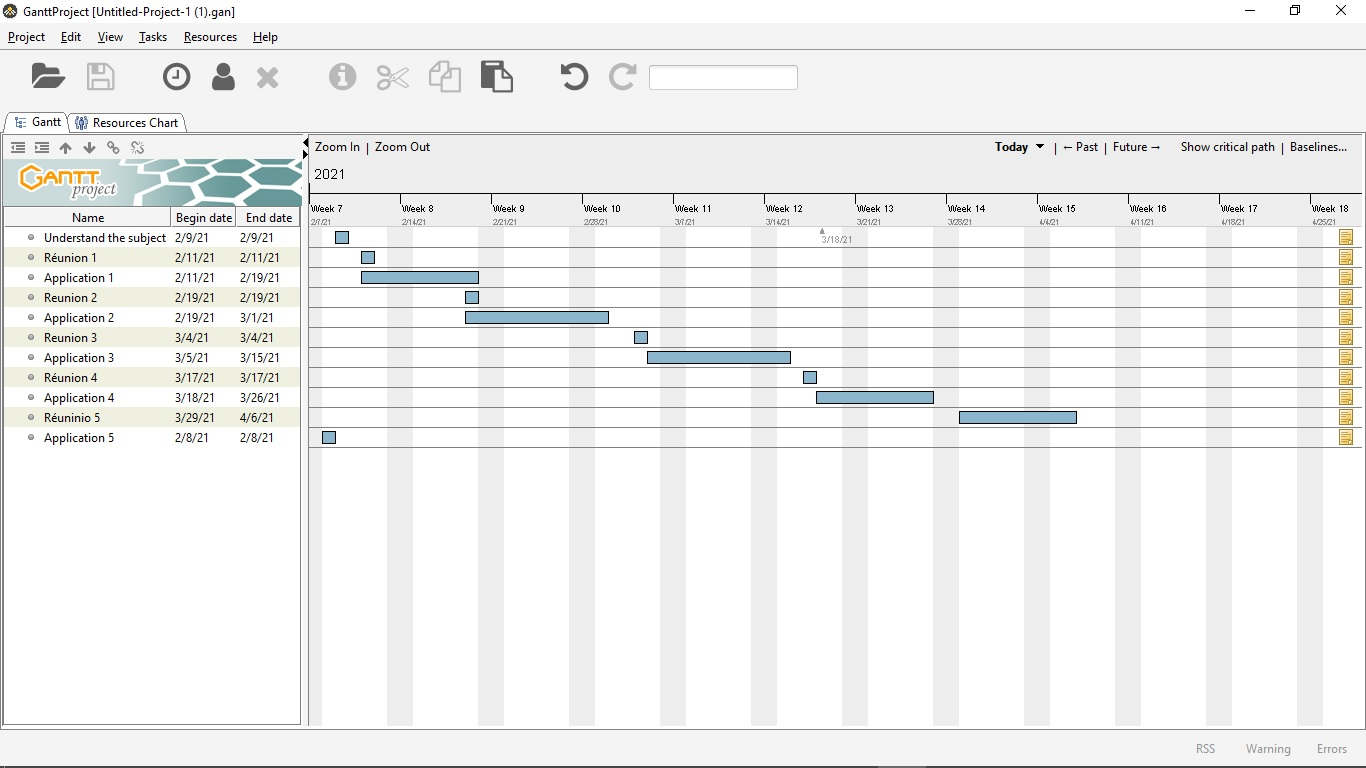
\includegraphics[width=100mm]{GG.jpg}
\caption{Project Planning Course \label{overflow}}
\end{figure}

\end{document}
